\section{Deelvraag 2: Architectuur}
In deze paragraaf zijn de resultaten voor deelvraag 2 \textit{\SubquestionTwo} verzameld en geanalyseerd.
Er is samen met de architect van het CMS Erwin Keuning en met software engineer Kevin Snijder een IT archtecture sketching sessie gedaan.
In deze sessie is de huidige softwarearchitectuur inbeeldt gebracht en is er ook aandacht besteed aan het in beeld brengen van het datamodel.
Verder is er ook gebruik gemaakt van interne documentatie van het systeem om de tekeningen te onderstuenen.
De diagrammen zijn afgeleid van de originele tekeningen die gemaakt zijn tijdens de sessie deze tekeingen zijn te vinden in Bijlage \ref{appendix:ITArchitectureSketch}.

% \todo[inline]{interne documenten toevoegen als data verzamle stukje)}

\subsection{Systeem}
Het eerste gedeelte van het IT Architecuture sketching is besteed aan het globale systeem / flow van het systeem.
Er zijn op dit moment 3 verschillende Snakeware Cloud site methodes deze methodes zijn XSL \Parencite{XSL}, Vue 2 en Vue 3 \Parencite{Vue} site.
De Vue 2 en 3 werken door middel van de Snakware Cloud API en de XSL werkt door middel van de Snakeware.Site code base.
In afbeelding \ref{fig:SystemArchitectureXSL} is te zien hoe de XSL sites werken, in afbeeldingen \ref{fig:SystemArchitectureVue} is te zien hoe de vue sites werken.

\whitespace
Het Snakeware Cloud platform zelf is een XSL site dat aangepast kan worden door middel van het CMS (dit wordt alleen nooit gedaan).
Er wordt gebruik gemaakt van stored procedures om de data op te halen van de database, deze data wordt automatisch omgezet naar XML.
De XML wordt getransformeerd in bruikbare JSON format \Parencite{JSON} in het geval van de Vue 2 en 3 sites, en in het geval van een XSL site wordt het getransformeerd naar javascript en HTML \Parencite{HTML}.
deze data wordt vervolgens gebruikt om de data te tonen op de frontend.

\whitespace
\begin{graphic}
	\captionsetup{type=figure}
	\caption{Globale systeemarchitectuur XSL sites}
	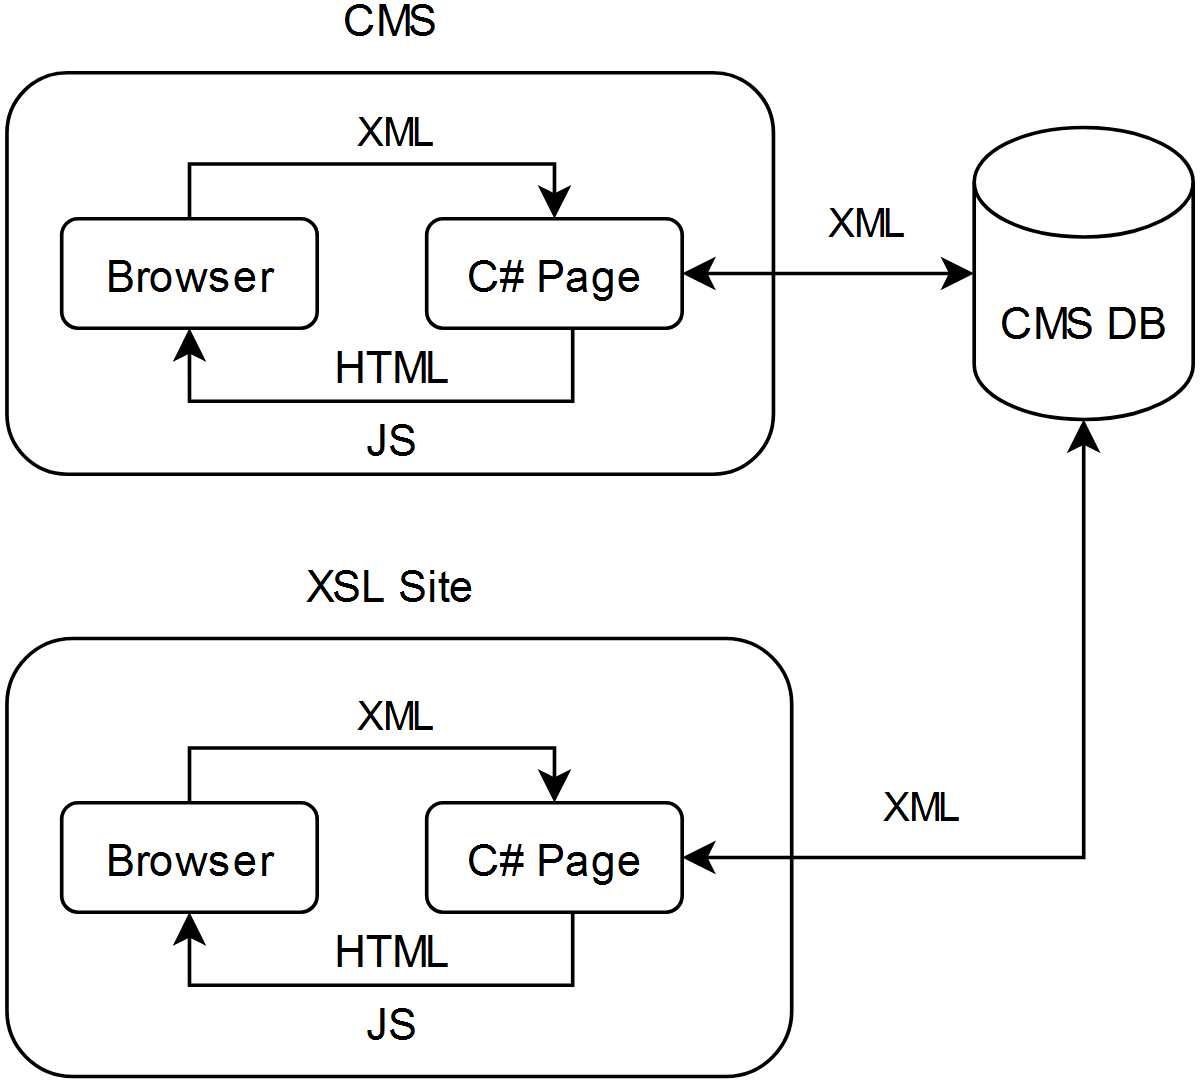
\includegraphics[scale=0.4]{XSLCMS}
	\label{fig:SystemArchitectureXSL}
\end{graphic}

% \whitespace
\begin{graphic}
	\captionsetup{type=figure}
	\caption{Globale systeemarchitectuur Vue 2 en 3 sites}
    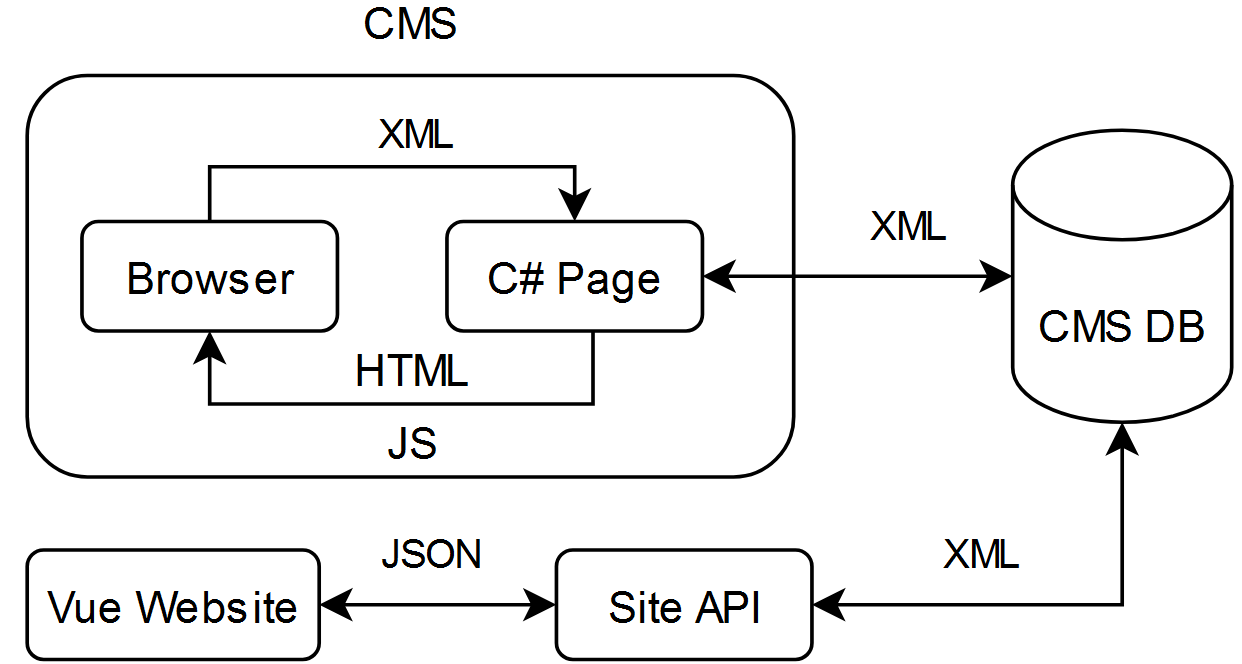
\includegraphics[scale=0.4]{VueCMS}
	\label{fig:SystemArchitectureVue}
\end{graphic}

% \todo[inline]{Maak hier van een deployment diagram of package diagram van zodat het UML is}
% \todo[inline]{Leg meer uit wat XSL XML en JSON HTML is}

\whitespace
Tijdens de IT Architeture sketching was er ook ruimte overgelaten om te onderzoeken waar er mogelijk verbeteringen gemaakt konden worden.
Uit de persoonlijke communicatie met Erwin en Kevin zijn de volgende punten uit gekomen.

\begin{itemize}
	\item[-]{Het Huidige \gls{CMS} maakt geen gebruik van de SOLID principes, dit zorgt er voor dat het moeilijk te testen en uit te breiden is van wege de interconnected code}
	\item[-]{Het \gls{CMS} is op dit moment een grote monoliet, dit brengt problemen met zich mee rond het schalen van het systeem.}
	\item[-]{Het is momenteel niet realistische om het \gls{CMS} te testen door middel van unit testen, dit is echter wel gewild.}
    \item[-]{Veel van de logica van het CMS zit vastgekoppeld in de frontend, en dit is niet gewild.}
\end{itemize}

\newpage
\subsection{Het datamodel}
Het volgende onderdeel is het schetsen van het datamodel, dit is ook gedaan samen met Erwin en Kevin.
Op dit moment maakt het \gls{CMS} gebruik van 288 tabellen, deze tabellen bevatten meerdere kolommen en zijn interconnected.
Daarom is er tijdens de het schetsen van het datamodel alleen gekeken naar de belangrijkste tabellen en de relaties hier tussen.
De exacte data dat opgeslagen wordt in deze tabellen weg gelaten om het overzichtelijk te houden.
Het versimpelde datamodel van het CMS is te zien in figuur \ref{fig:DatamodelCMS}.

\begin{graphic}
	\captionsetup{type=figure}
	\caption{Gesimplificeerde datamodel CMS}
	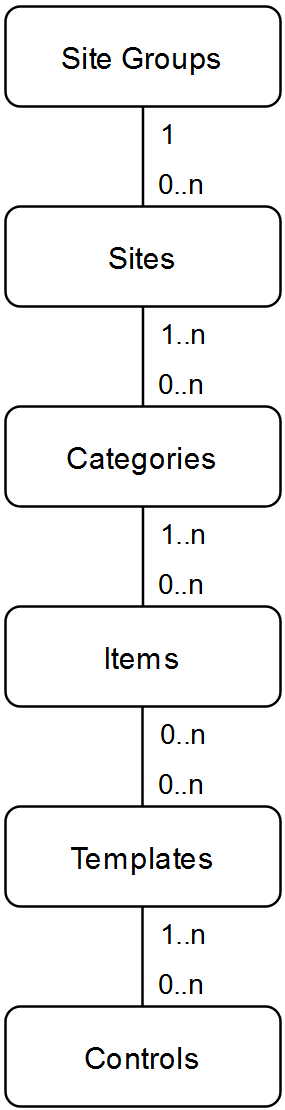
\includegraphics[scale=0.5]{DatamodelCMS}
	\label{fig:DatamodelCMS}
\end{graphic}

\whitespace[2]
Na het schetsen van het datamodel is er gevraagt waar op dit moment de meeste problemen worden gevonden in het datamodel.
Deze punten zijn verzameld tijdens de sessie door middel van persoonlijke communicatie met Erwin en Kevin.
\begin{itemize}
    \item[-]{Het datamodel is erg complex, dit maakt het lastig om nieuwe functionaliteiten in het CMS te bouwen}
    \item[-]{Het datamodel heeft te veel connecties met andere tabellen terwijl dit niet nodig zou moeten zijn.
        Dit maakt het systeem onnodig complex.}
    \item[-]{De huidige naamgeving van de tabbellen en kolommen is niet als gewild.
        Als we dit nu aan zouden passen dan zorgt dit problemen in de code maar met een nieuw project zouden we graag andere naamgeving willen hebben.}
\end{itemize}

\whitespace
Tijdens de sessie kwam er naar voren dat mensen binnen het R\&D uitgesproken meningen hebben ov er een nieuw datamodel.
Hierom wordt er een sessie gepland tijden de ontwerpfase met het R\&D team om mogelijk tot een consensus te komen over een geschikt model.
% Een van de grotere problemen met het datamodel is dat het \textbf{erg complex} is (persoonlijke com erwin) dit maakt het lastig om nieuwe functionaliteiten in het CMS te bouwen.
% Het datamodel heeft relaties die niet kloppen en kunnen mogelijk voor problemen zorgen (pc kevin).
% Dit zorgt er voor dat het CMS lastig uit te breiden is en veel tijd kost om te onderhouden.
% Tijdens de sessie kwam naar voren dat mensen een uitgesproken meening hebben over een nieuwe datamodel.
% Hierom wordt er een sessie gepland na het onderzoeks verslag tijdens de ontwerp fase met het R\&D team om mogelijk tot een consencus te komen over een geschikt model.
%
%
% Het geeft de inpressie dat het datamodel veel \qw{on nodige relaties heeft}, verder is de naam geving de colommunen niet meer van deze tijd (pc Erwin).
%
% \todo[inline]{Ik ben de netwerk opstelling vergeten in het onderzoek om mee te nemen kan dit gezien als een mogelijke verbetering.}
% Een van de grote problemen nu met het huidige CMS is dat het niet gebruikt maakt van de SOLID prinicples (Personelijke cummunicatie erwin).
% Ook is het CMS een grote Monolith dit zorgt er voor dat het niet goed schaalt met meerdere gebruikers (Persoonlijke communicatie kevin).
%
% \whitespace
% Verder wordt er nog steeds gebruik gemaakt van XML als data transfer object, dit is niet optimaal in de loop der jaren zijn er andere varianten gekomen die hier beter voor geschikt zijn.
% In de huidige code base door de verbondenheid van het systeem is het niet practies om het CMS te unit testen (PC Kevin), en dit willen we wel graag.
% Hiernaast is er ook nog aandacht besteed aan de huidige netwerk opstelling van Snakeware.
% Door middel van de interne documentatie.
% \todo[inline]{Verbeter de teksten}
% \todo[inline]{Opzoeken hoe je persoonlijke communicatie refereerd}
